\documentclass[10pt,letterpaper]{article}
\usepackage[top=0.85in,left=2.75in,footskip=0.75in]{geometry}
\usepackage{bibentry}

% Text layout specific to Supplemental Materials
\topmargin 0.0cm
\oddsidemargin 0.5cm
\evensidemargin 0.5cm
\textwidth 16cm
\textheight 21cm

\setlength{\parskip}{1em}

% Template for PLoS
% Version 3.2 March 2016

% General commands for text/figures

% Page margin
\usepackage[top=0.85in,left=2.75in,footskip=0.75in]{geometry}
% Use Unicode characters when possible
\usepackage[utf8x]{inputenc}
% amsmath package, useful for mathematical formulas
\usepackage{amsmath}
%\usepackage{natbib}
% amssymb package, useful for mathematical symbols
\usepackage{amssymb}
%\usepackage{booktabs}
\usepackage{xspace}
\usepackage{hyperref}
% graphicx package, useful for including eps and pdf graphics
% include graphics with the command \includegraphics
\usepackage{graphicx}

% Use adjustwidth environment to exceed column width (see example table in text)
\usepackage{changepage}

% textcomp package and marvosym package for additional characters
\usepackage{textcomp,marvosym}

% fixltx2e package for \textsubscript
\usepackage{fixltx2e}

% cite package, to clean up citations in the main text. Do not remove.
\usepackage{cite}
\usepackage{caption}
\usepackage{subcaption}
\usepackage{rotating}

\usepackage{color}

% Use doublespacing - comment out for single spacing
%\usepackage{setspace}
%\doublespacing


% Bold the 'Figure #' in the caption and separate it with a period
% Captions will be left justified
\usepackage[labelfont=bf,labelsep=period,justification=raggedright]{caption}

% Use the PLoS provided bibtex style
%\bibliographystyle{/Users/stephens/Dropbox/Documents/stylefiles/plos2009}

% Remove brackets from numbering in List of References
\makeatletter
\renewcommand{\@biblabel}[1]{\quad#1.}
\makeatother

% Use nameref to cite supporting information files (see Supporting Information section for more info)
\usepackage{nameref,hyperref}

% line numbers
%\usepackage[right]{lineno}

% ligatures disabled
\usepackage{microtype}
\DisableLigatures[f]{encoding = *, family = * }

% Leave date blank
\date{}

%\pagestyle{myheadings}
%% ** EDIT HERE **
\usepackage{enumerate}
\usepackage{multirow}
\usepackage{url}
\usepackage{xr} %for cross-referencing
%% ** EDIT HERE **
%% PLEASE INCLUDE ALL MACROS BELOW
\newtheorem{algorithm}{Algorithm}
\newtheorem{proposition}{Proposition}
\newtheorem{restateproposition}{Proposition}
\newtheorem{lemma}{Lemma}
\newtheorem{corollary}{Corollary}
\newtheorem{result}{Result}
\newtheorem{note}{Note}
\newtheorem{definition}{Definition}

\def\KL{\text{KL}}

% Text layout
\raggedright
\setlength{\parindent}{0.5cm}
\textwidth 5.25in
\textheight 8.75in

% Bold the 'Figure #' in the caption and separate it from the title/caption with a period
% Captions will be left justified
\usepackage[aboveskip=1pt,labelfont=bf,labelsep=period,justification=raggedright,singlelinecheck=off]{caption}
\renewcommand{\figurename}{Fig}

%------ bibliography
% Use the PLoS provided BiBTeX style
\bibliographystyle{bmc-mathphys}
% Remove brackets from numbering in List of References
\makeatletter
\renewcommand{\@biblabel}[1]{\quad#1.}
\makeatother


%% Author's settings
\def\KL{\text{KL}}

\pagestyle{empty} %%in order to delete the number at the bottom of the page


\begin{document}
\section*{Supplementary Figures}
\newpage

\begin{figure*}[h!]
\centering
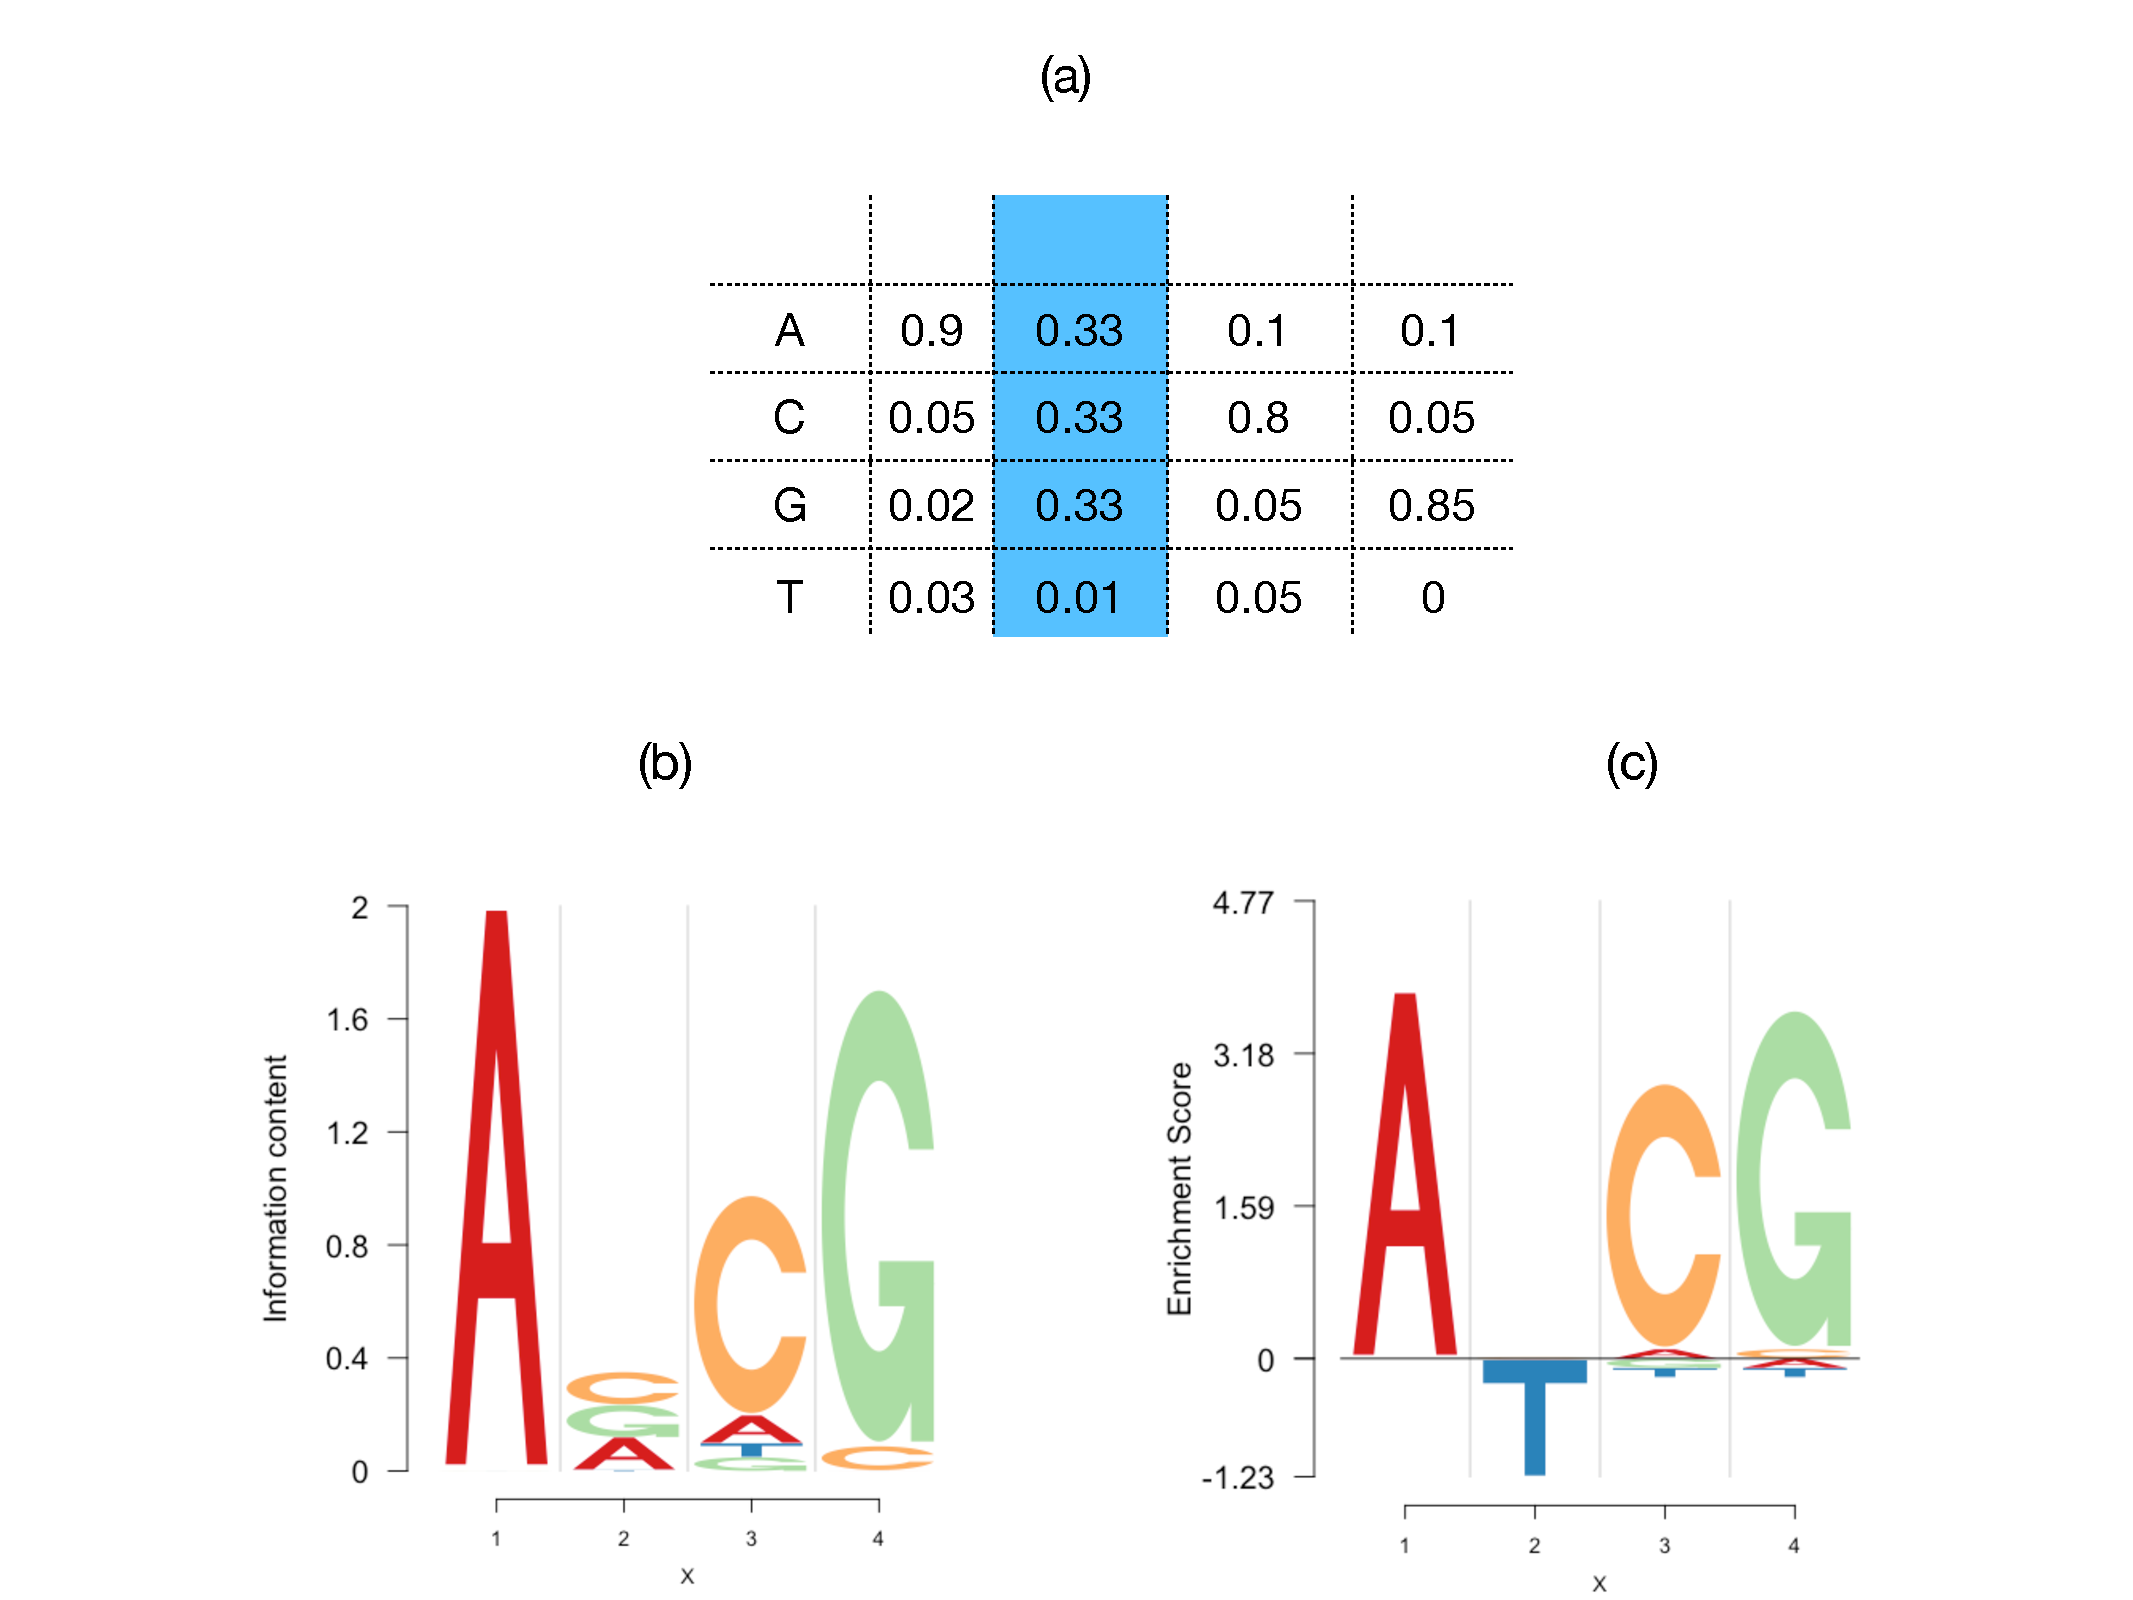
\includegraphics[height=6in, width=7in]{figures2.split/figures2_2.pdf}
\caption{ \textbf{Illustration of the EDLogo representation.}
      We present an illustration of how \textit{EDLogo} representation accounts for depletion signal and provides a more informative visualization of the sequence motif. In panel (a), we present a position weight matrix with the position weight vector at the second position having a depletion of $T$, but is flanked by enrichments around it. In panel (b), we present the corresponding standard logo plot representation of the PWM matrix in panel (a). The signal at the second position gets swamped by the bias towards enrichment signals flanking it. In panel (c), we present the \textit{EDLogo} representation of the PWM matrix, where both the enrichment signals as well as the depletion signal at position 2 are clearly observed.}
\label{fig:suppfig1}
\end{figure*}


\begin{figure*}[h!]
\centering
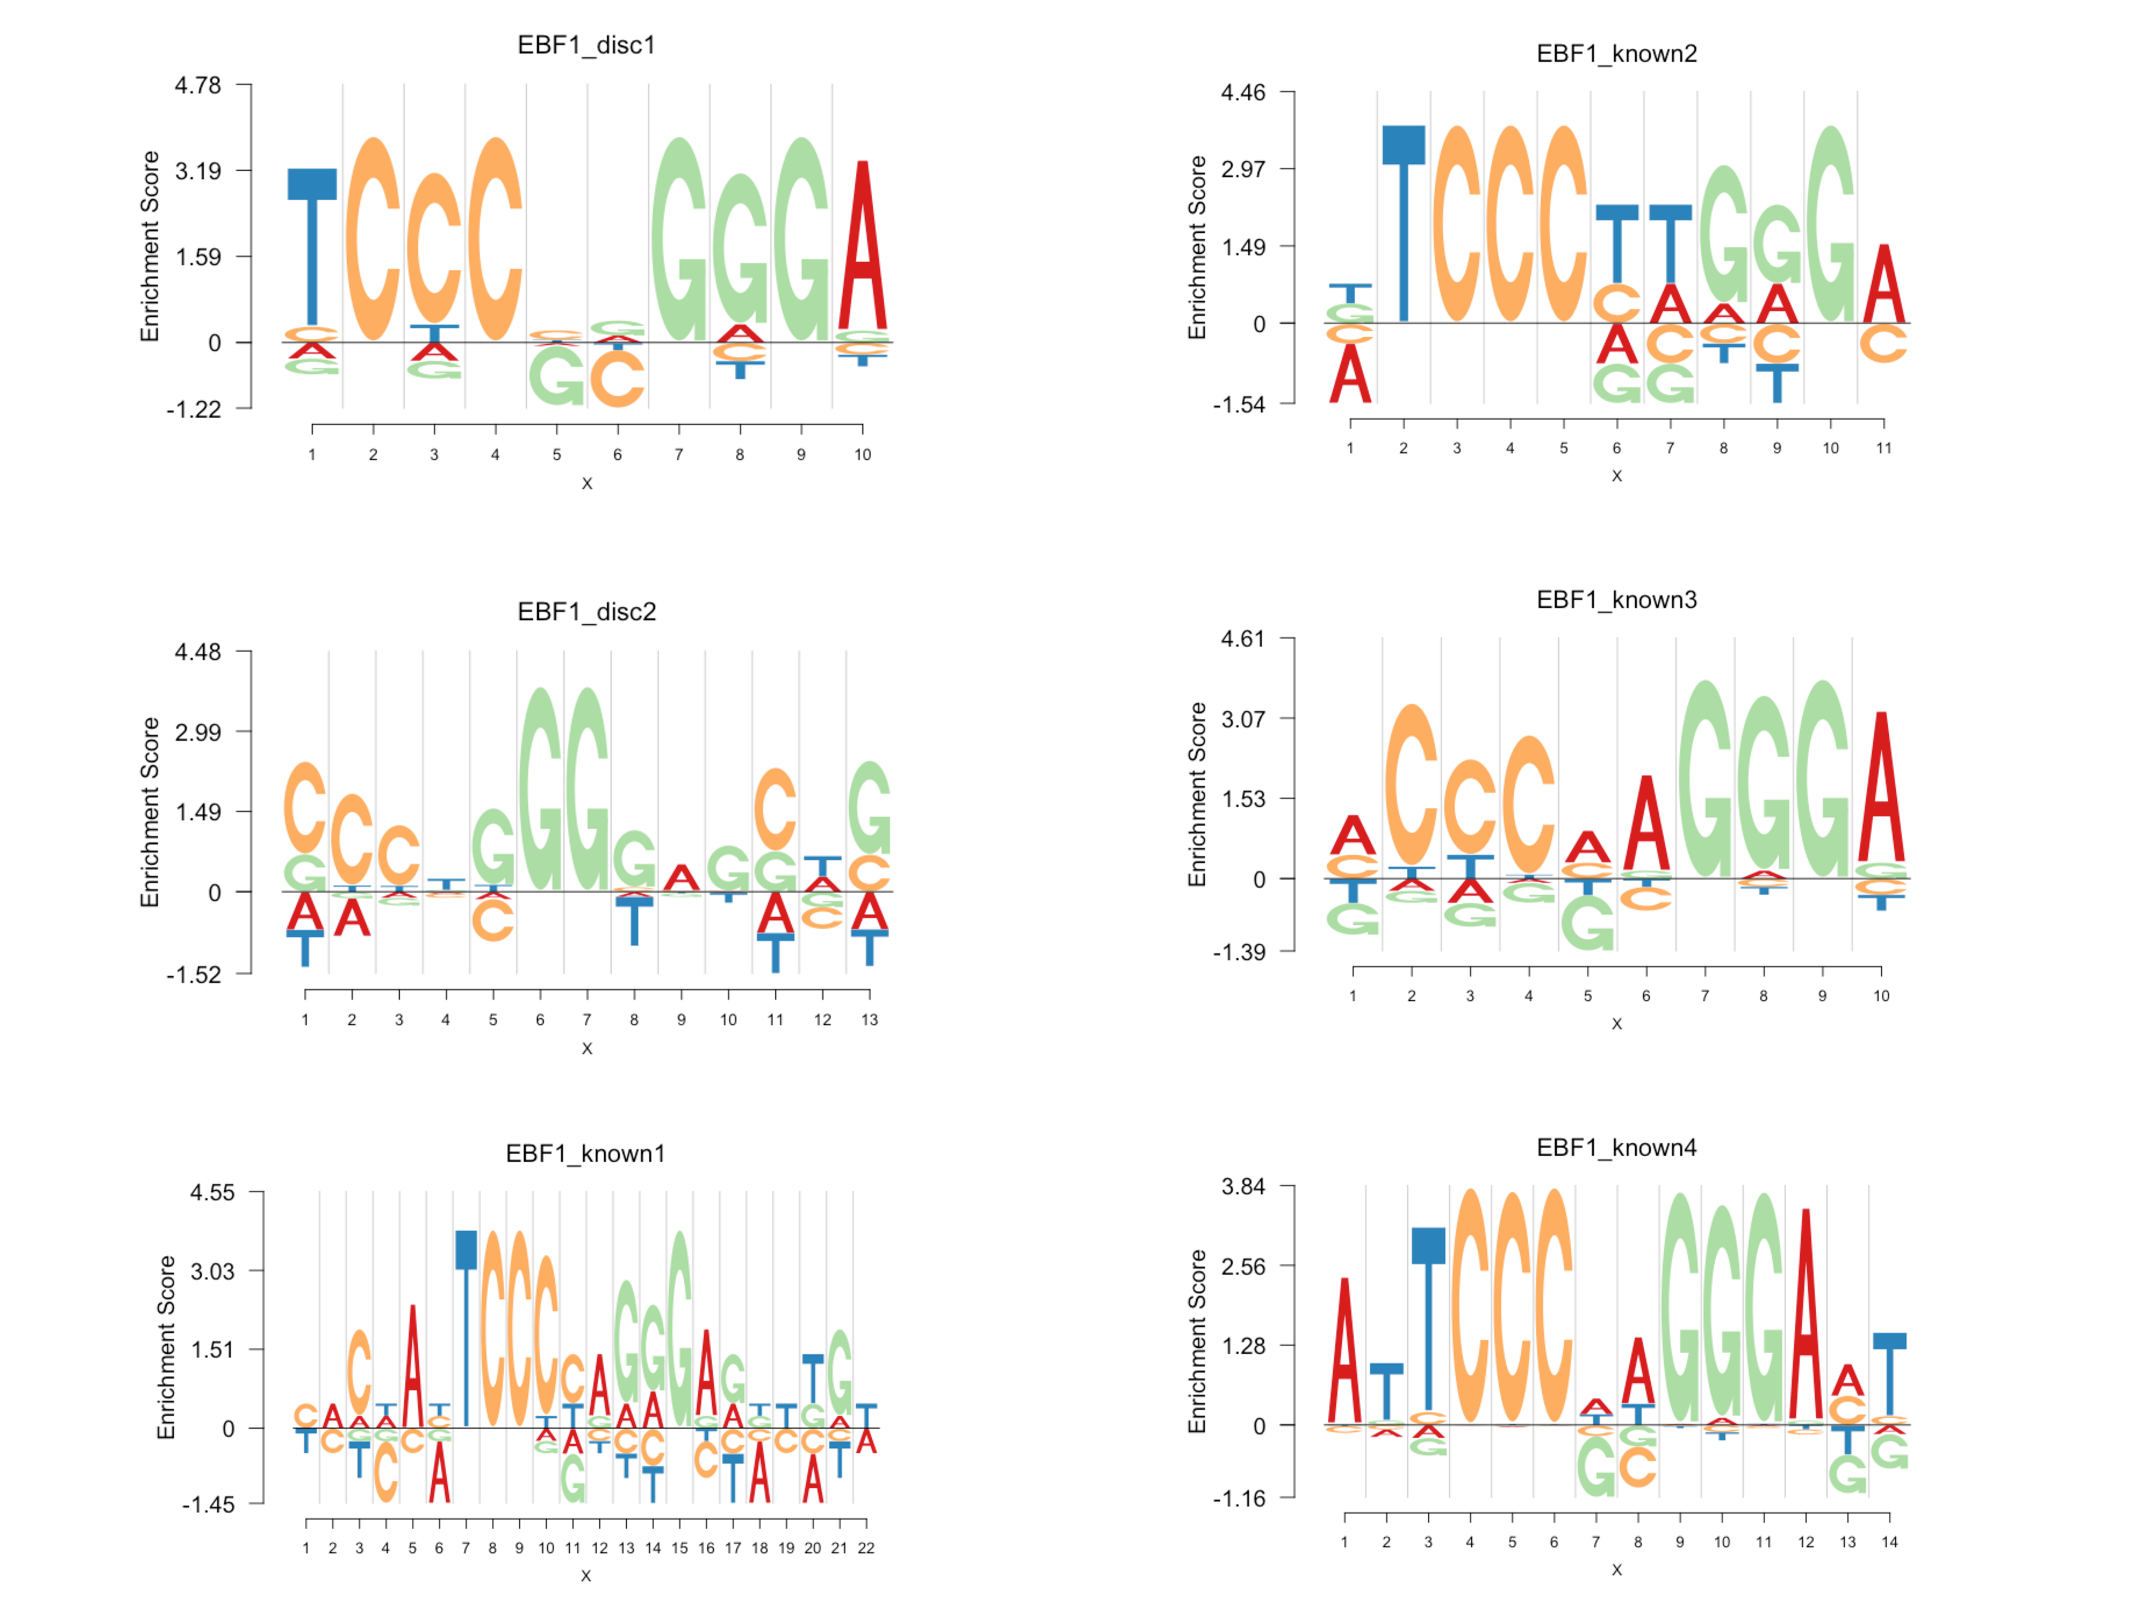
\includegraphics[height=6in, width=7in]{figures2.split/figures2_3.pdf}
\caption{\textbf{EDlogo representation of the members of the EBF1 family of transcription factors}: We present the \textit{EDlogo} representation for the binding sites of 6 transcription factors in the EBF1 family. EBF1-known4 and EBF1-disc1, and also to some extent EBF1-known3 seem to show the depletion of G and C in the middle of the binding site. The PWM data for all the transcription factors have been obtained from the ENCODE TF Chip-seq datasets and are hosted on the webpage \url{http://compbio.mit.edu/encode-motifs/} \cite{Kheradpour2013}.}
\label{fig:suppfig2}
\end{figure*}

\begin{figure*}[h!]
\centering
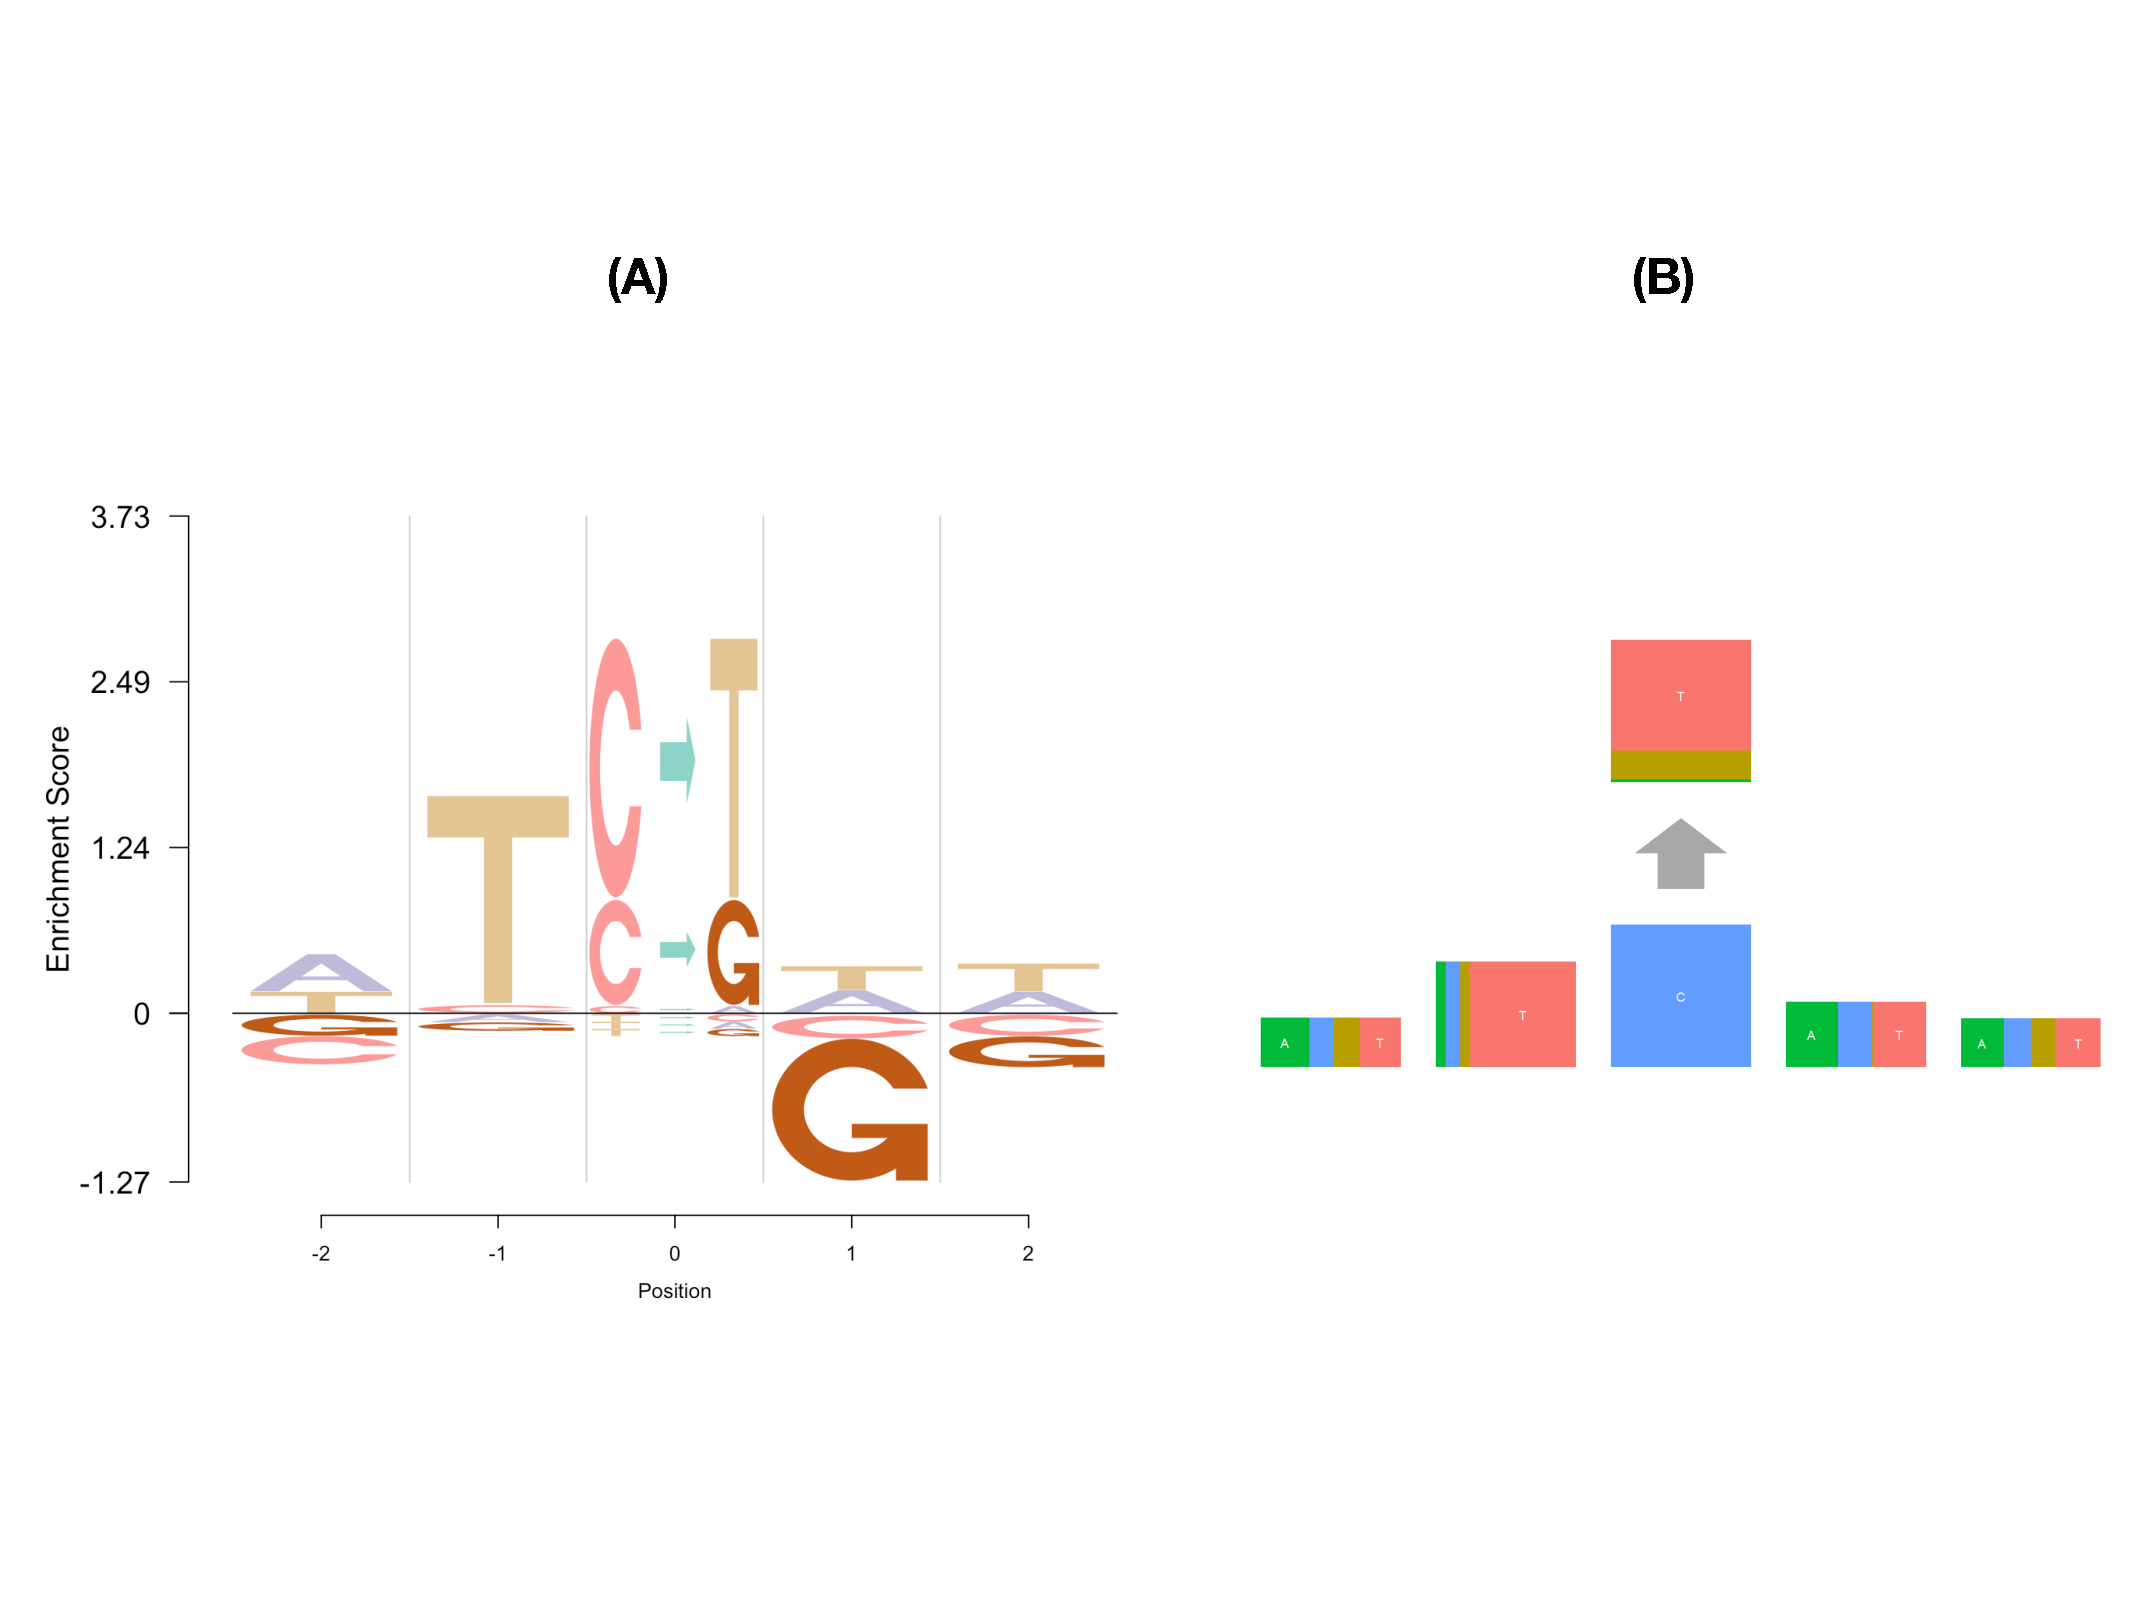
\includegraphics[height=6in, width=7in]{figures2.split/figures2_4.pdf}
\caption{\textbf{Comparison of Logolas EDLogo plot with pmsignature representation for cancer mutation signatures}: 
We compare the \textit{EDLogo} plot representation and the \textit{pmsignature} representation due to Shiraishi et al (2015) \cite{Shiraishi2015} for mutation signature profile of lymphoma B cell from Alexandrov et al 2013 \cite{Alexandrov2013}. The position 0 corresponds to the mutation. Positions $-1$ and $-2$ correspond to the the two left flanking bases with respect to the mutation. Positions $1$ and $2$ correspond to the the two right flanking bases with respect to the mutation. Clearly, \textit{EDLogo} representation shows the depletion of G at the right flanking base more clearly and is more interpretable and visually appealing in highlighting the overall mutation signature patterns compared to the\textit{pmsignature} plot.}
\label{fig:suppfig3}
\end{figure*}

\begin{figure*}[h!]
\centering
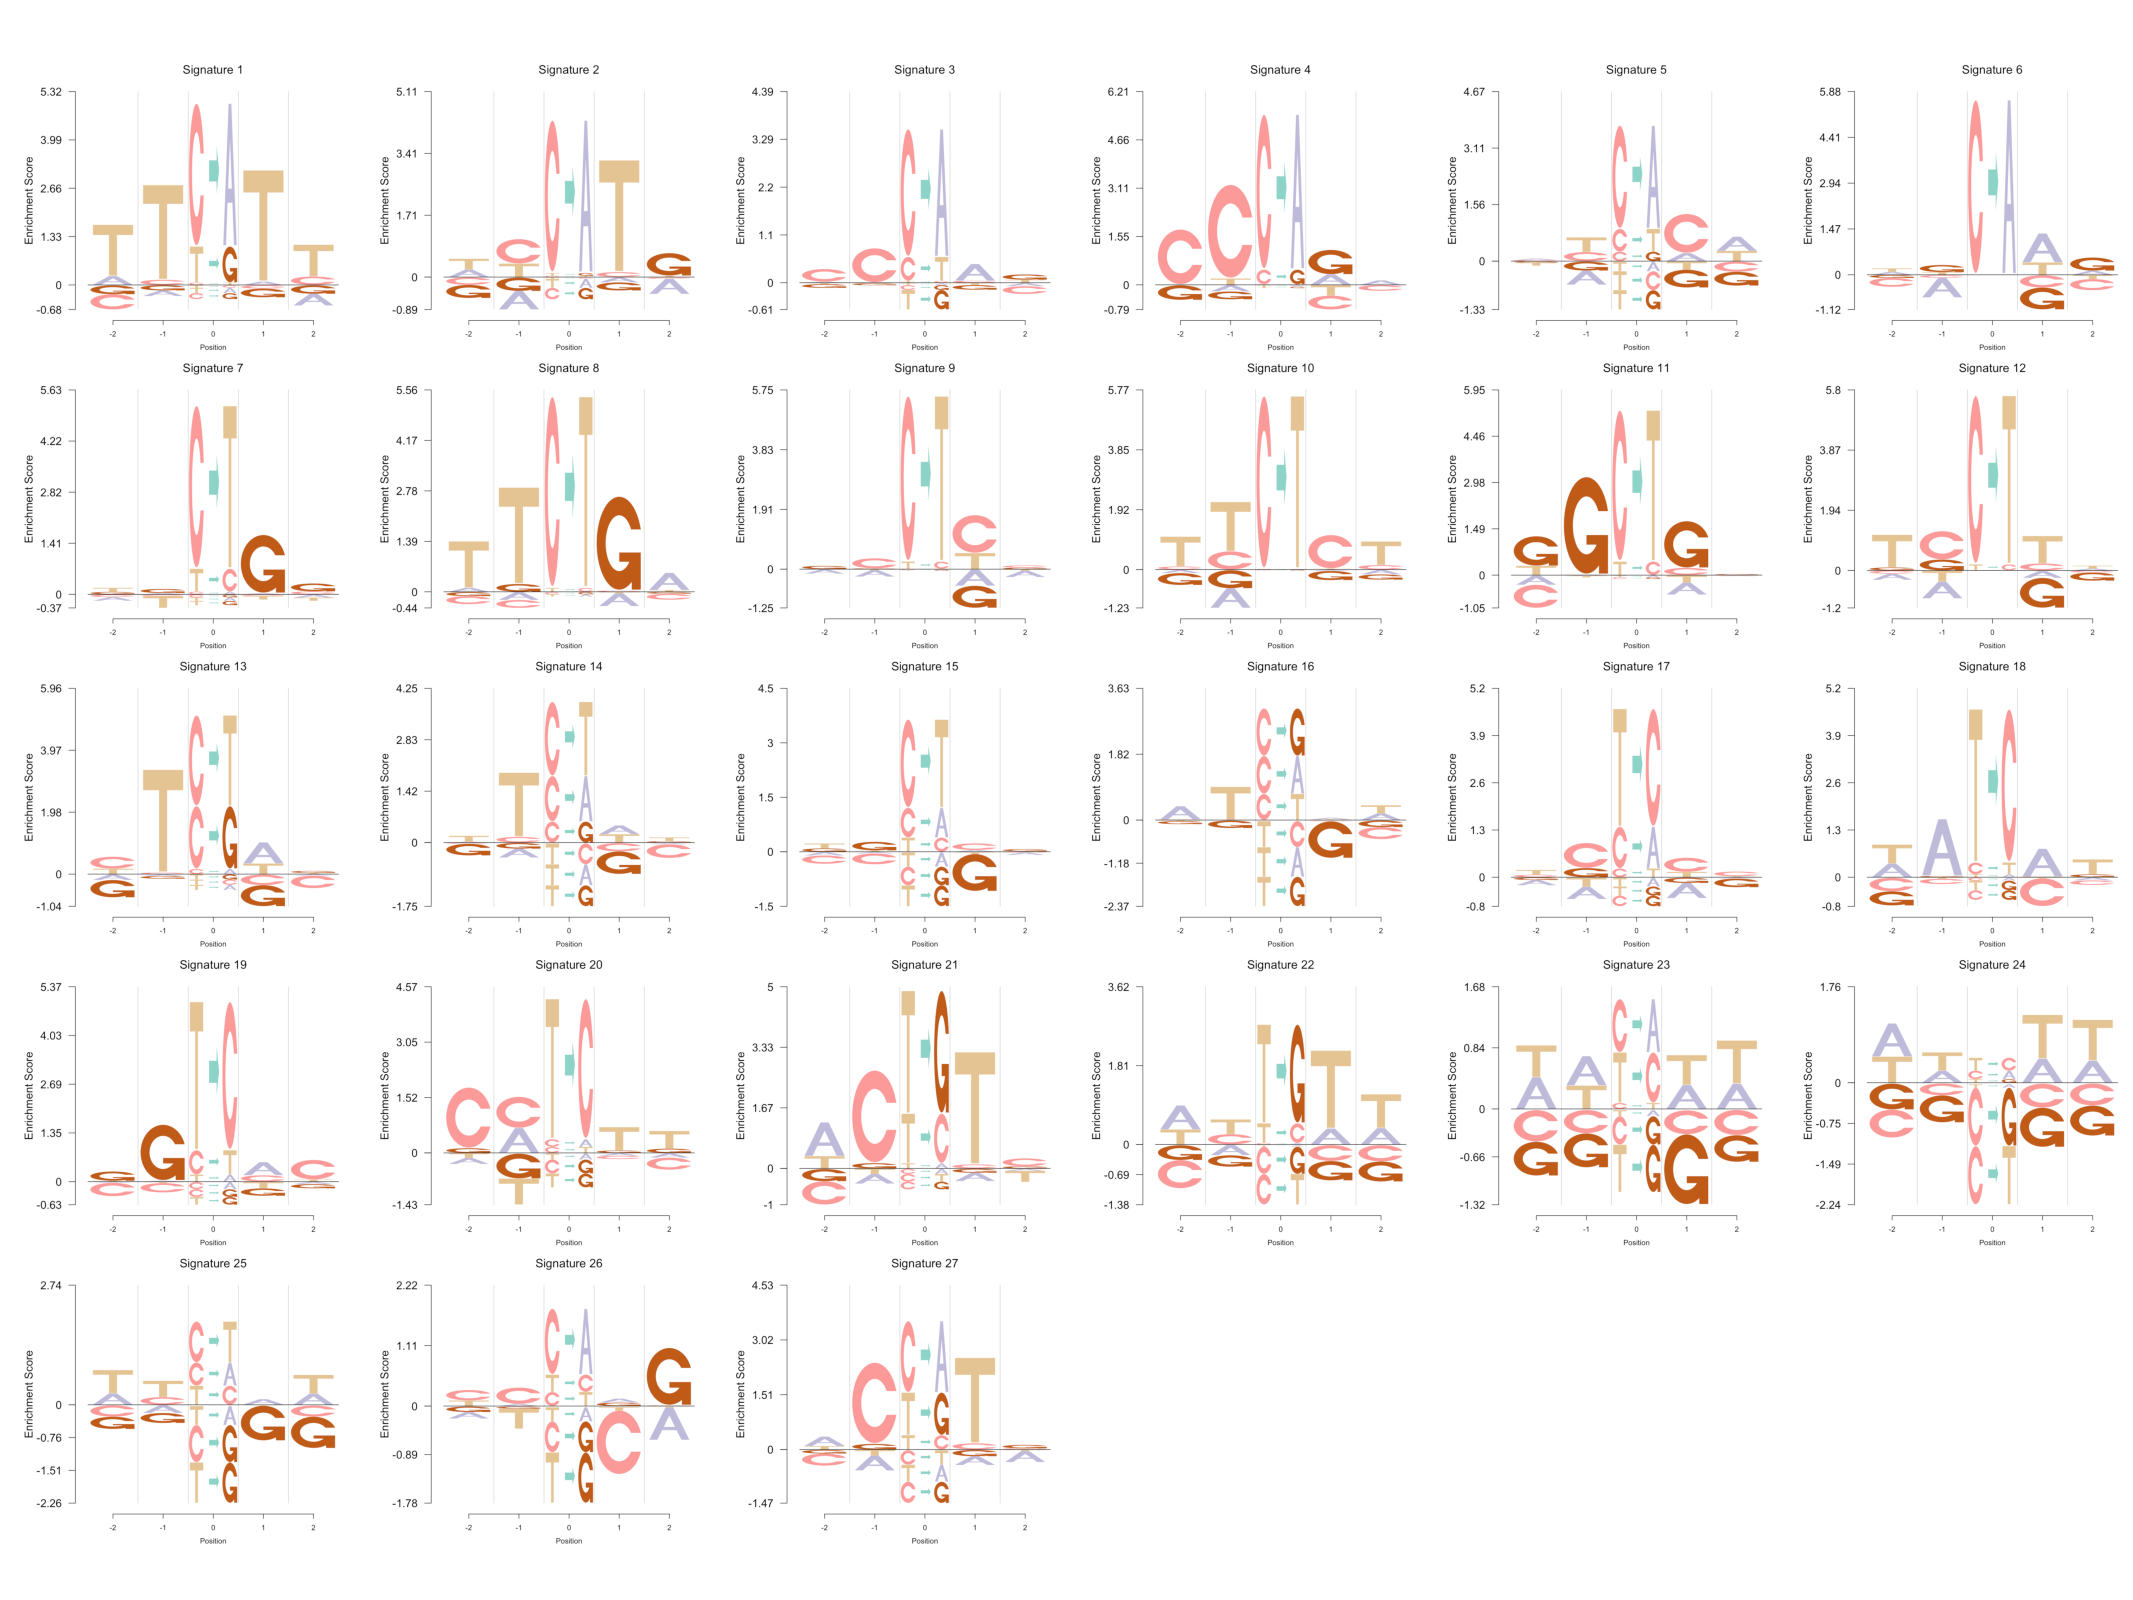
\includegraphics[height=6in, width=7in]{figures2.split/figures2_5.pdf}
\caption{\textbf{EDLogo plots for the mutational signature profiles for 27 clusters in Shiraishi et al (2015)}: 
We present the \textit{EDlogo} representations (ratio) method for the 27 cluster signature profiles obtained from fitting a grade of membership model on the cancer mutational signature data across 30 cancer types by Shiraishi et al (2015) \cite{Shiraishi2015}. This plot is an alternative logo plot based representation of Figure 4 in Shiraishi et al (2015) \cite{Shiraishi2015}.}
\label{fig:suppfig4}
\end{figure*}

\begin{figure*}[h!]
\centering
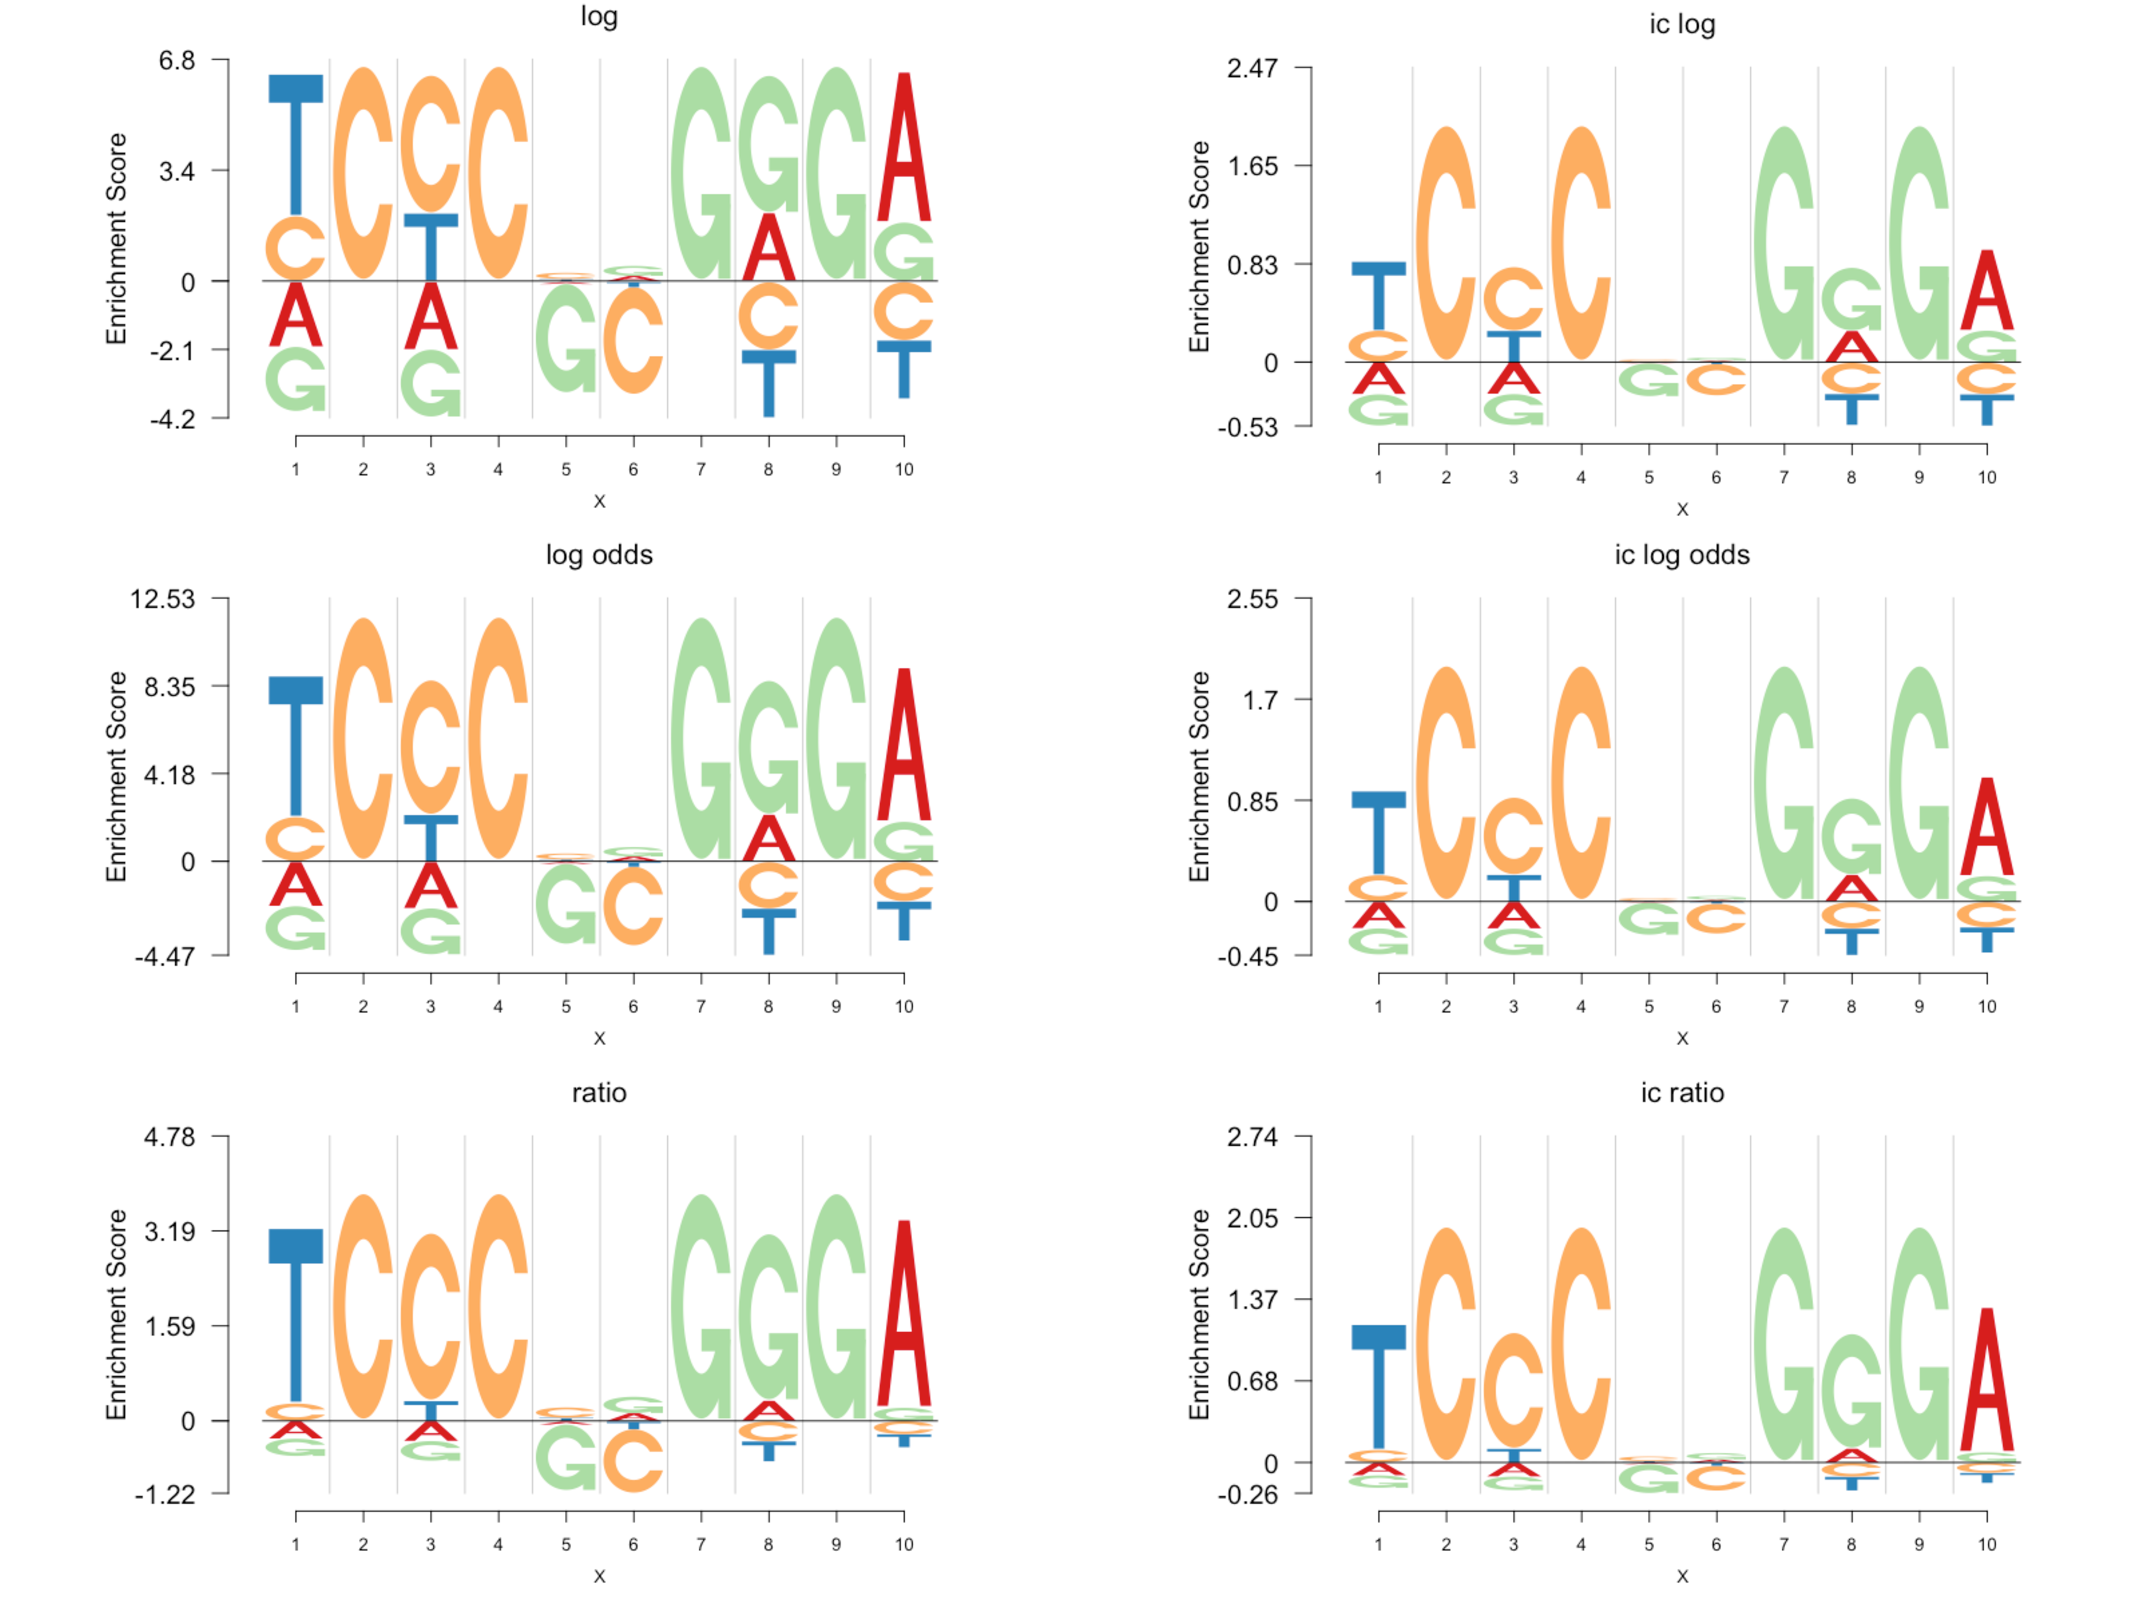
\includegraphics[height=6in, width=7in]{figures2.split/figures2_6.pdf}
\caption{\textbf{Different options for EDLogo representation - TFBS example}: We present the visualizations corresponding to the different options of the \textit{EDLogo} plot for the EBF1-disc1 transcription factor. The details of the methods behind the various options of \textit{EDLogo} are presented in Supplementary Methods.}
\label{fig:suppfig5}
\end{figure*}

\begin{figure*}[h!]
\centering
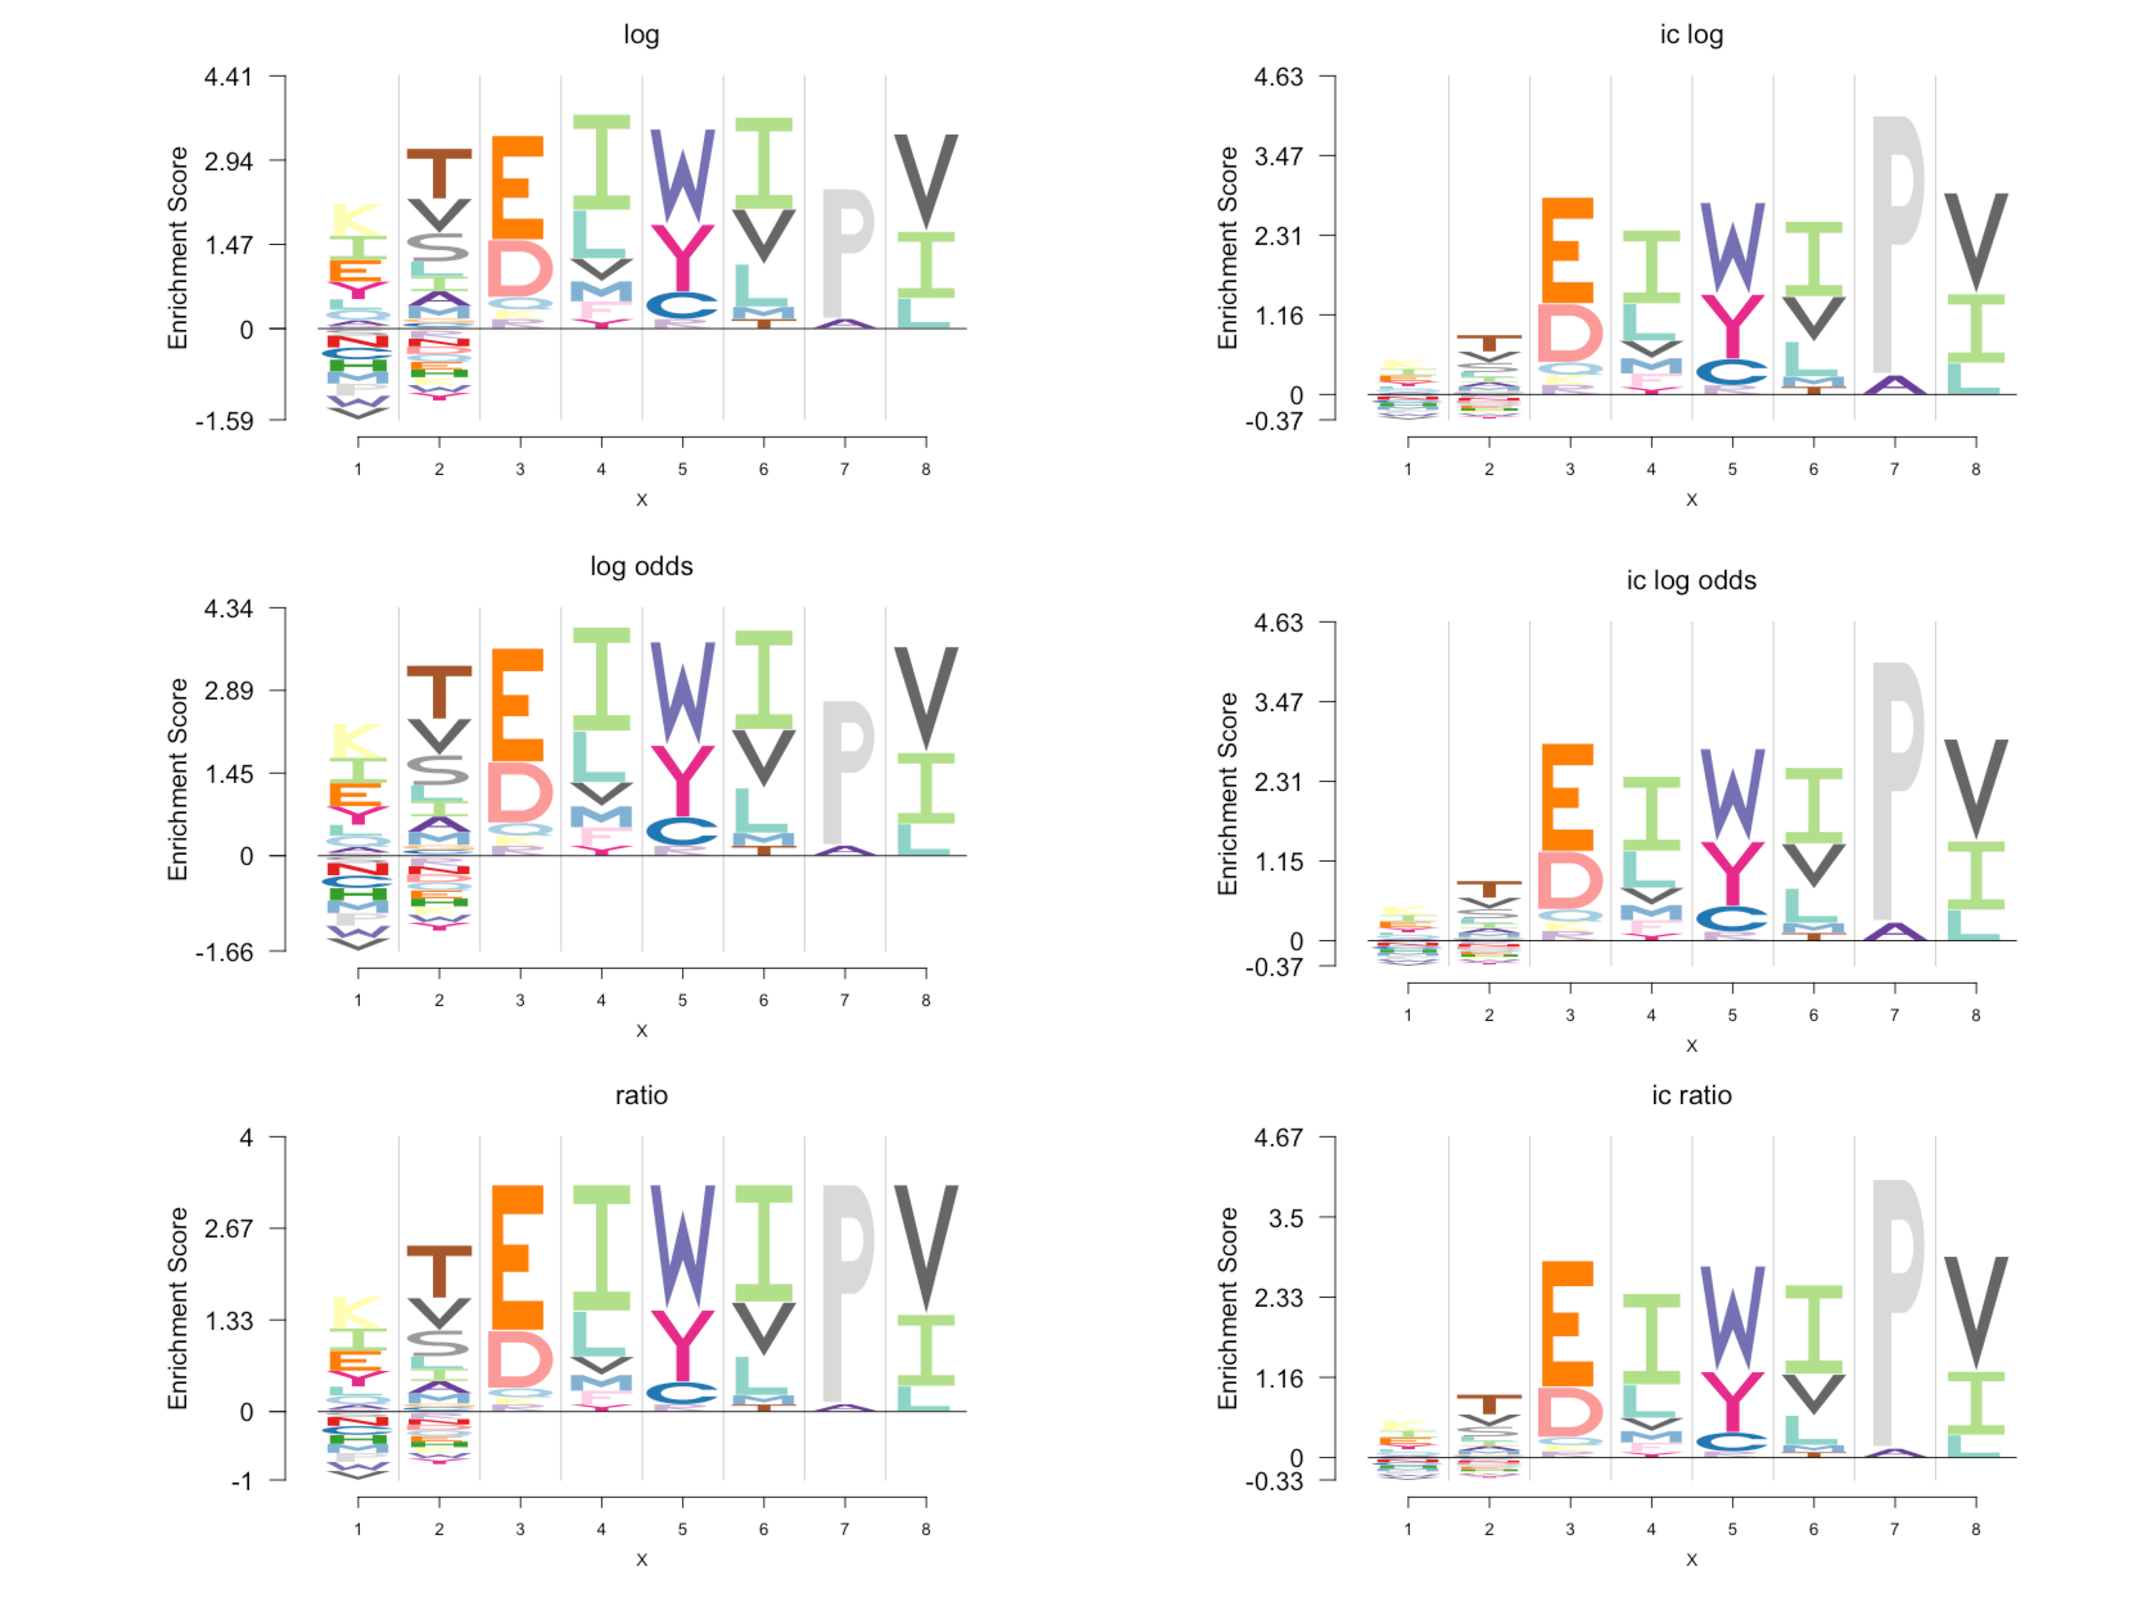
\includegraphics[height=6in, width=7in]{figures2.split/figures2_7.pdf}
\caption{\textbf{Different options for EDLogo representation - Protein example}: We present the visualizations corresponding to the different options of the \textit{EDLogo} plot for the binding sequence of the Bacterial transcription activator, effector binding domain protein PF06445 (motif 4, Start=153 Length=8).}
\label{fig:suppfig6}
\end{figure*}


\begin{figure*}[h!]
\centering
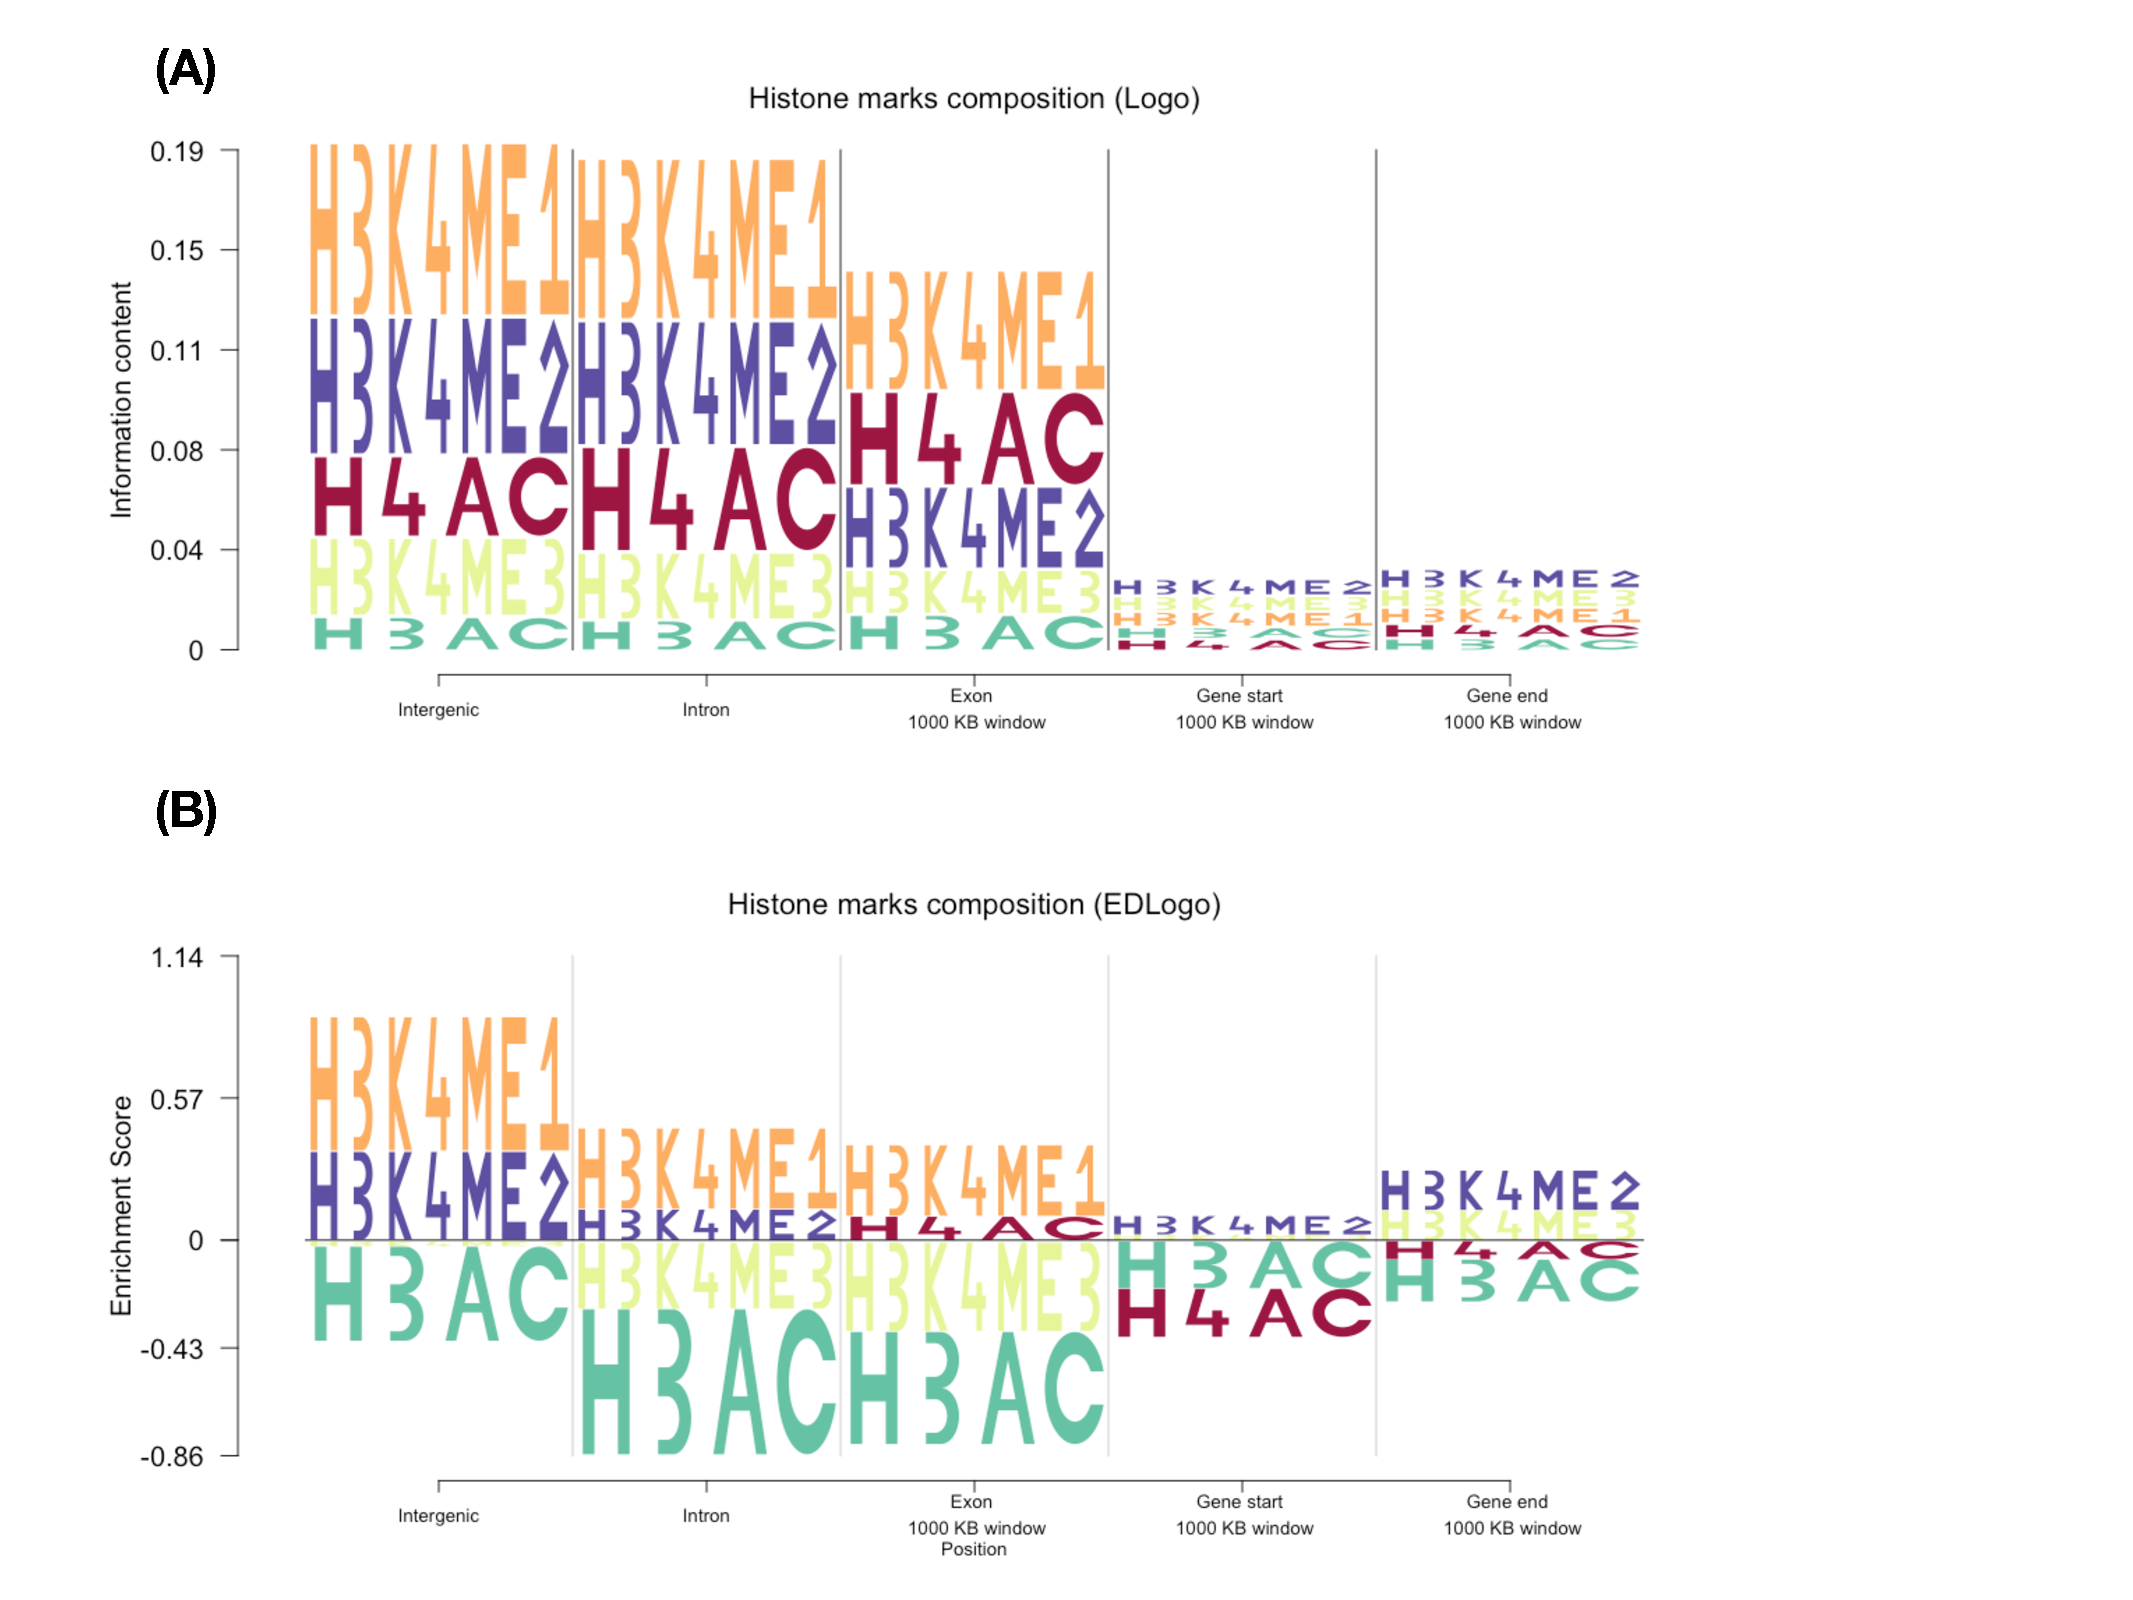
\includegraphics[height=6in, width=7in]{figures2.split/figures2_8.pdf}
\caption{ \textbf{Example applications of string logo plots.}
We present the standard and the \textit{EDlogo} plot representations of the composition of histone modification types that overlap with an intergenic region, intron, exon, gene start or gene end for the lymphoblastoid cell line GM06990 as reported in Koch et al 2007 \cite{Koch2007}. These plots use alphanumeric string symbols as characters in the plot - a special feature of the package \textit{Logolas}.}
\label{fig:suppfig6}
\end{figure*}

\end{document}
